\begin{displayquote}
	\textsf{After the validation of the numerical and parallel performance of $m$-UCGLE, a major difficulty to profit from UC methods including $m$-UCGLE is to implement the manager engine which can well handle their fault tolerance, load balance, asynchronous communication of signals, arrays and vectors, the management of different computing units such as GPUs, etc. In the last chapter, we tried to give a naive implementation of the engine to support the management tasks on the homogeneous platforms based on MPI\_SPAWN and MPI non-blocking sending and receiving functionalities. The stability of this implementation of the engine cannot always be guaranteed. Thus we are also thinking about to select the suitable workflow/task based environments to manage all these aspects in the UC approach. YML\footnote{http://yml.prism.uvsq.fr/} is a good candidate, which is a workflow environment to provide the definition of the parallel application independently from the underlying middleware used. The special middleware and workflow scheduler provided by YML allows defining the dependencies of tasks and data on the supercomputers \cite{delannoyyml}. YML, including its interfaces and compiler to various programming languages and libraries, will facilitate the implementation of UC based methods with different numerical components. In this chapter, firstly we summarize the YML framework, and then analyze the limitations of existing YML implementation for UC approach. In the end, we propose the solution.}
\end{displayquote}

\vspace{1in}


\section{YML Framework}
YML is a workflow environment dedicated to the execution of parallel de distributed applications on various middleware. The YML framework enables the description of the complex parallel application based on the tasks. The task-based application written based on YML language can be executed on several runtime-systems or middleware without changes. YML is a software layer between the end-user and the runtime system of a supercomputer and/or the middleware of a distributed system, which is in charge of communication. YML is composed of three main parts: an IDL, a kernel and a back-end allowing interactions with the runtime-system or middleware. A high-level workflow language, a just-in-time scheduler and a system of service integration constitute the kernel of YML. The high-level language which is XML-based permits the description of the graph of application. The nodes of the graph correspond to computation while edges correspond to dependencies or communications. A component could be itself a graph. The language integrates the ability to describe components on the one hand and application graphs on the other hand. Both aspects are encapsulated in XML document for homogeneity. This language provides a way to specify the communication between components during the execution of the application. The graph can contain parallel and sequential sections and standard construction of most languages including branching, exceptions, and loops. The graph language describes the dependencies between the components during the execution. These dependencies rest on the notion of events. The compiler translates the graph of components of applications in an internal representation containing a set of components calls. The scheduler manages application execution and acts as a client for the underlying runtime system accurately requiring computing resources. During the application execution, the scheduler detects tasks ready for execution solving dependencies at runtime. Each scheduling step may or may not generate a set of parallel tasks, which are translated in computing requests to runtime system through dedicated backends. A service in YML can be “any kind” of a component such as a library (or some component of), a data repository, or a catalog of binary components. Thanks to the component-oriented design of YML, it is easy to incorporate new ones. The computation components can be written in different programming languages like XMP. In the case of using XMP in YML, the tasks, written in XMP are expected to be executed on sub-clusters or groups of nodes, which are tightly connected. These tasks would be hybrid programs with distributed and shared programming models. The scheduler provided by YML invokes and manages the tasks among the sub-clusters or
groups.

Environments such as YML, allowing the realization of the proposed model must be extensible in all their aspects and offer reusability. Furthermore, the ability thereof to provide dynamic integration of end-users expertise is a significant element.

\subsection{YML Design}

The aim of YML is to provide users with an easy-of-use method to run parallel applications on different Grid platform and supercomputer. The framework can be divided into three parts which are the end-users interface, frontend, and backend. The end-users interface is used to provide an easy-to-use and an intuitive way to submit their applications and applications can be described using a workflow language YvetteML, Frontend is the main part of YML which includes a compiler, scheduler, data repository, abstract and implementation components.

Abstract and implementation components based on function can be reused. The backend is the part to connect different Grid and peer to peer middleware.

The development of a YML application is based on the components approach, and then we will discuss the three kinds of components in detail.

\begin{itemize}
	\item \textbf{Abstract component} defines the communication interface with the other components. This definition gives the name, and the communication channels correspond to a data input, data output or both and are typed. This component is used in the code generation step and to create the graph.
	
	\item \textbf{Implementation component} is the implementation of an abstract component. It provides the description of computations through YvetteML language. The implementation is done by using common languages like C or C++. They can have several implementations for the same abstract component.
	
	\item \textbf{Graph component} carries a graph expressed in YvetteML instead of a description of computation. It provides the parallel and sequential parts of an application and the synchronization events between dependent components. It is a straightforward way for scientific researchers to develop their application.
\end{itemize}

Moreover, those three components are independent of middleware. So, to run an application on another grid environment with a different middleware, the user needs to compile each component for the middleware of his choice. OmniRPC as the backend of YML will be used here.

YML helps the developer in the whole process of parallelizing applications. It starts at the early stage of components creation to the execution of hardly constrained workflow applications on a Grid. Moreover, YML allows the test and validation of those applications on the user computer using a special backend which relies on the multithreading capabilities of the underlying operating system.

YML eases components creation. Existing code can be reused by importing libraries as some new components without any adaptation. Those components are called by the application when computational tasks have to be started. Moreover, the notions of abstract and implementation descriptions of components bring three interesting features for the Grid scheduler that can be included in the framework.

\begin{itemize}
	\item \textbf{data migration} can be easily quantified at the start and at the end of the application thanks to the abstract definition.
	\item \textbf{data used} by a component is clearly defined in the abstract and implementation definitions, therefore this can be used in a checkpointing feature to move a component from a node to an other.
	\item \textbf{computation time} of a component can be evaluated thanks to the implementation definition.
\end{itemize}

The use of Data Repository Servers hides the data migrations to the developer and ensure that necessary data are always available to all components of the application.

\begin{figure}[htbp]
	\centering
	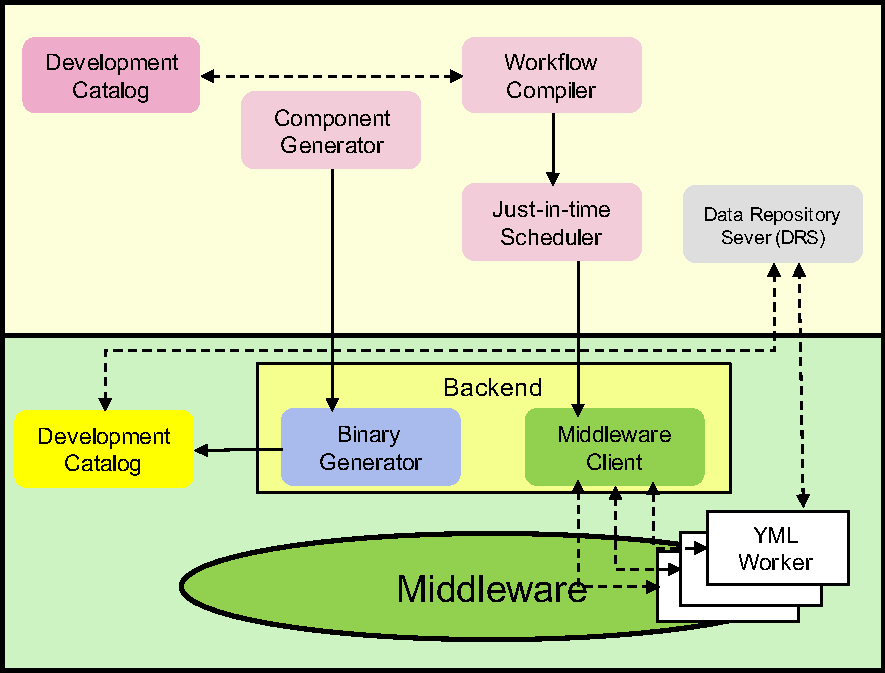
\includegraphics[width=.92\linewidth]{fig/yml-arch.pdf}
	\caption{YML Architecture.}
	\label{yml-arch}
\end{figure}

\subsection{Yvette Language}

\begin{itemize}
	\item \textbf{Parallel Section:} par section 1 // ... // section N endpar
	\item \textbf{Sequential loop:} seq (i:=begin;end) do ... enddo
	\item \textbf{Parallel loop:}  par (i:=begin;end) do ... enddo
	\item \textbf{Conditional structure:} if (condition) then ... else ... endif
	\item \textbf{Synchronization:} wait(event) / notify(event)
	\item \textbf{Component call:} compute NameOfComponent(args,...,...)
\end{itemize}

\subsection{YML Example}

\begin{figure*}[htbp]
	\centering
	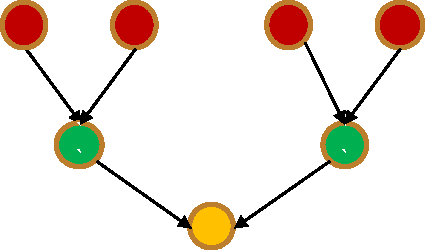
\includegraphics[width=3.in]{fig/sum_workflow.pdf}
	\caption{Workflow of Sum Application.}
	\label{fig:sum_workflow}
\end{figure*}

\subsubsection{Abstract}

\lstset{language=XML}
\begin{lstlisting}[frame=single]
<?xml version="1.0" encoding="utf-8"?>
<component type="abstract" name="test_abstract"
           description="sum of two doubles">
    <param type="real" mode="out" name="res" />
    <param type="real" mode="in" name="a" />
    <param type="real" mode="in" name="b" />
</component>
\end{lstlisting}

\subsubsection{Implementation}

\lstset{language=XML}
\begin{lstlisting}[frame=single]
<?xml version="1.0" encoding="utf-8"?>
<component type="impl" name="test_impl"
          description="sum of two doubles">
    <impl lang="CXX" libs="">
        <header><![CDATA[
          #include <stdlib.h>
        ]]>
        </header>
        <source lang="CXX" libs="">
          res = a + b;
        </source>
        <footer></footer>
    </impl>
</component>
\end{lstlisting}

\subsubsection{Application}

\lstset{language=XML}
\begin{lstlisting}[frame=single]
<?xml version="1.0" encoding="utf-8"?>
<application name="test_app">
    <description>
        sum application
    </description>
    <params></params>
    <graph>
       compute test(res, 1.0, 2.0); #res = 3.0
       compute test(res, results, results); #res = 6.0
    </graph>
</application>
\end{lstlisting}

\subsection{Multi-level Programming Paradigm: YML/XMP}

The multi-level programming paradigm YML/XMP is supported by the OmniRPC-MPI Middleware. OmniRPC is a thread-safe remote procedure call (RPC) system, based on Ninf, for cluster and grid environment. It supports typical master/worker grid applications. Workers are listed in a XML file named as the host file. For each host, the maximum number of job, the path of OmniRPC, the connecion protocol (ssh, rsh) and the user can be defined.

An OmniRPC application contains a client program which calls remote procedures through the OmniRPC agent. Remote librairies which contain the remote procedures are executed by the remote computation hosts, there are implemented like a executable program which contains a network stub routine as its main routine. The declaration of a remote function of remote library is defined by an interface in the Ninf interface definition language (IDL). The implementation can be written in familiar scientific computation language like FORTRAN, C or C++.

There are two versions of OmniRPC, one is for grid computation and the other for supercomputer. The first one (the original version) was designed for the grid computing and distributed architecture of large numbers of computers. The second one was created specially for supercomputers, the XMP language is only usable with this version of OmniRPC if we want to use YML in complement.


\begin{figure}[htbp]
	\centering
	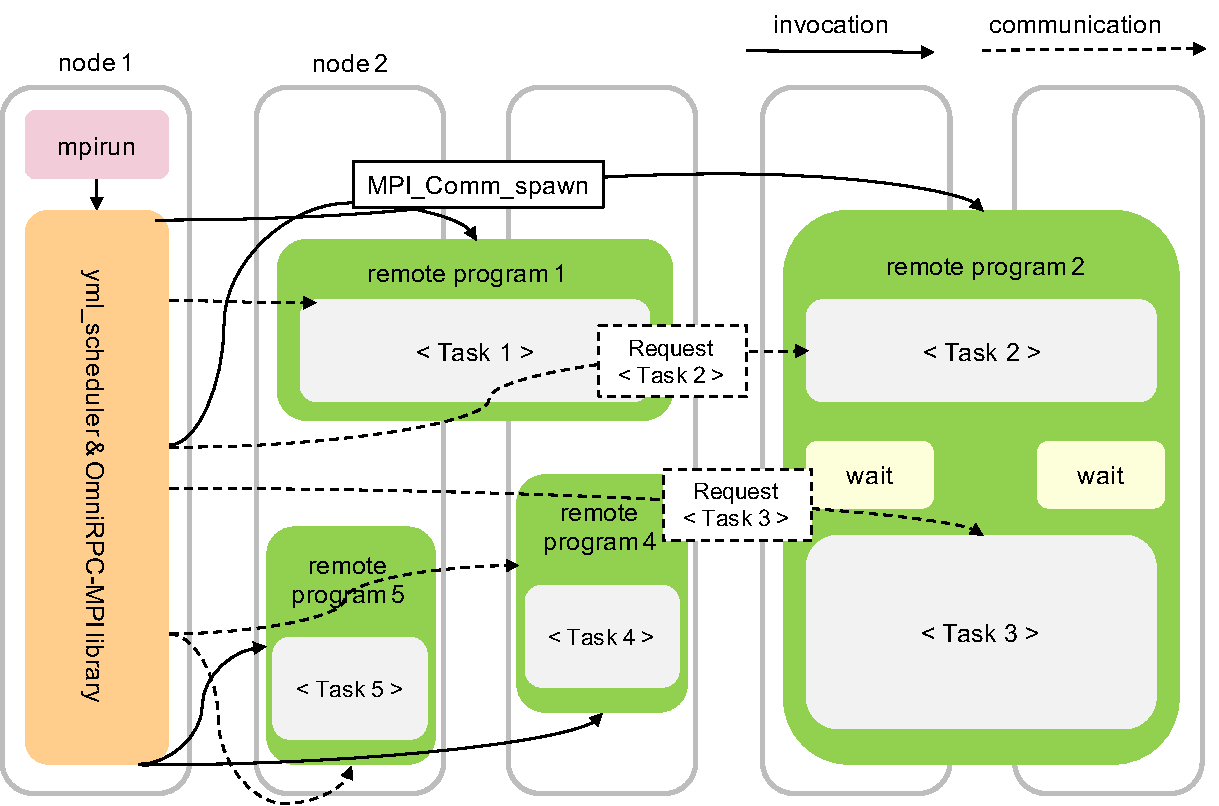
\includegraphics[width=.92\linewidth]{fig/xmp-yml-exec.pdf}
	\caption{Application Execution with YML + OmniRPC-MPI.}
	\label{xmp-yml-exec}
\end{figure}


\section{Limitations of YML for UC Approach}

\subsection{Workflow of $m$-UCGLE Analysis}


\begin{figure}[htbp]
	\centering
	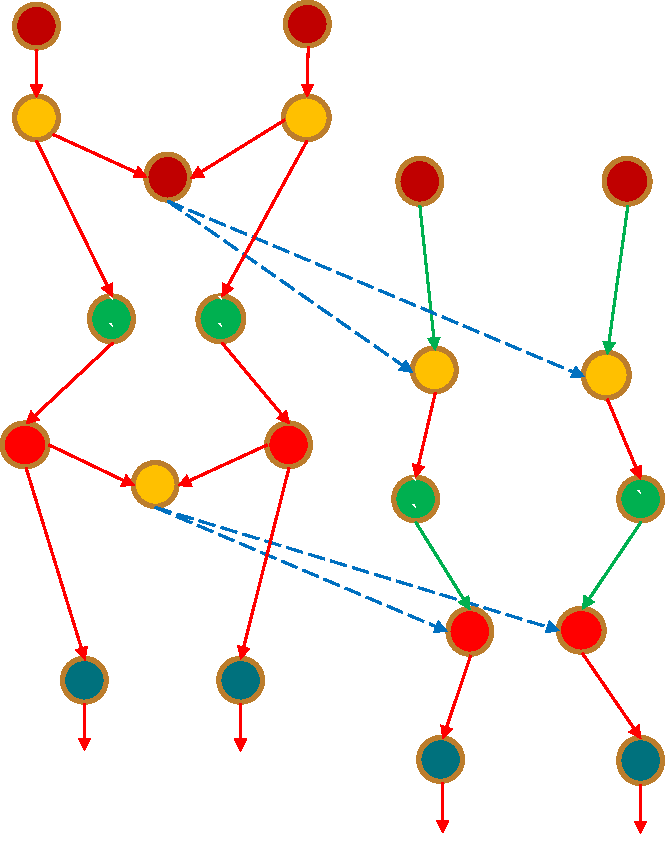
\includegraphics[width=3.8in]{fig/m-UCGLE-task.pdf}
	\caption{m-UCGLE task.}
	\label{m-UCGLE-task}
\end{figure}


\subsection{Mechanism for Convergence}
\subsection{Asynchronous Communications}
\section{Proposition of Solution}

\subsection{Dynamic Graph Grammar in YML}

We want to have dynamic graphs. The graphs may depend of variable  modified into Implement components. Then, in Abstract components :

\lstset{language=XML}
\begin{lstlisting}[frame=single]
<param type="var_graph" mode="inout" name="foo">
\end{lstlisting}

The variable for the dynamic graph can be the mode of \textit{in}, \textit{out} or \textit{inout}. These parameter may be evaluated and modified on a task, or  only evaluate a logical  into Yvette “if (logical) then … else ..."; If the computation to evaluate the logical is to complex, we may use a task with a special indication, added on the Implementation component, such as “graph\_scheduler\_evaluation”  : then the scheduler may manage those tasks as others, of run it “itself”.

\subsubsection{Scenario Example}

As shown in Fig. \ref{fig:sum_workflow2}. The red and purple are the addition operations, and the yellow point is the operation to set value. The priority of setting value is: 1) check the output value $a$ of red point, if this value is odd, then set the value to be $a$; 2) if $a$ is even, set the value to be $b$.

\begin{figure*}[htbp]
	\centering
	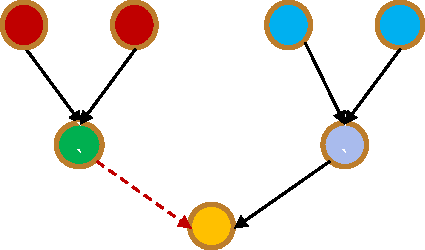
\includegraphics[width=3.in]{fig/sum_workflow2.pdf}
	\caption{New Scenario with Dynamic Graph.}
	\label{fig:sum_workflow2}
\end{figure*}

\subsubsection{Abstract}

\lstset{language=XML}
\begin{lstlisting}[frame=single]
<?xml version="1.0" encoding="utf-8"?>
<component type="abstract" name="dyntest_abstract"
          description="sum of two doubles #2">
    <param type="real" mode="out" name="val" />
    <param type="real" mode="in" name="a" />
    <param type="real" mode="in" name="b" />
    <param type="var_graph" mode="out" name="odd" /> 
</component>
\end{lstlisting}

\lstset{language=XML}
\begin{lstlisting}[frame=single]
<?xml version="1.0" encoding="utf-8"?>
<component type="abstract" name="dyntest_abstract"
          description="set value">
    <param type="real" mode="out" name="val" />
    <param type="real" mode="in" name="a" />
    <param type="var_graph" mode="inout" name="odd" /> 
</component>
\end{lstlisting}

\subsubsection{Implementation}

\lstset{language=XML}
\begin{lstlisting}[frame=single]
<?xml version="1.0" encoding="utf-8"?>
<component type="impl" name="dyntest_impl"
          description="sum of two doubles #2">
    <impl lang="CXX" libs="">
        <header><![CDATA[
          #include <stdlib.h>
        ]]>
        </header>
        <source lang="CXX" libs="">
           res = a + b;
           if(res % 2 ==0){
             odd = false;
           } else {
             odd = true;
           }
       </source>
       <footer></footer>
    </impl>
</component>
\end{lstlisting}

\lstset{language=XML}
\begin{lstlisting}[frame=single]
<?xml version="1.0" encoding="utf-8"?>
<component type="impl" name="setvalue_impl"
          description="set value">
    <impl lang="CXX" libs="">
        <header><![CDATA[
          #include <stdlib.h>
        ]]>
        </header>
        <source lang="CXX" libs="">
          val = a;
        </source>
        <footer></footer>
    </impl>
</component>
\end{lstlisting}

\subsubsection{Application}

\lstset{language=XML}
\begin{lstlisting}[frame=single]
<?xml version="1.0" encoding="utf-8"?>
<application name="dyntest_app">
    <description>
      set value application
    </description>
    <params></params>
    <graph>
      compute dyntest(res1, 1.0, 2.0, odd); #res = 3.0
      compute test(res2, 4.0, 6.0); #res = 10.0
      if(odd) then
         compute setvalue(val, res1, odd); #val = 3.0
      else
        compute setvalue(val, res2, odd); #val = 10.0
      endif
    </graph>
</application>
\end{lstlisting}


\subsection{Exiting Parallel Branch}

If the graph is dynamic and if we decide to exit a parallel branch:

\begin{itemize}
	\item we have to specify is all the running task as to be completed or not;
	\item we may want to finish all the task of the parallel branch before to exit;
	\item we may also decide to exit several level of parallelism;
	\item we may stop completely the computation.
\end{itemize}

Exit(level=p) : we exit p levels of parallelism (p loops if it is parallel loops)

Exit(complete=all) : all the running tasks of the level are finished (data?) before to exit

Exit(level=p,auto) : we add to each abstract components if the task has to be finished, data saved or not, if the task is running and we exit the parallel branch ( </exit finish = “yes” />  ) ; 
and we may ask in the asbtract component:

\lstset{language=XML}
\begin{lstlisting}[frame=single]
<param type="Matrix" mode="inout" name="A" save_exit="yes"/>
\end{lstlisting}

\begin{figure*}[htbp]
	\centering
	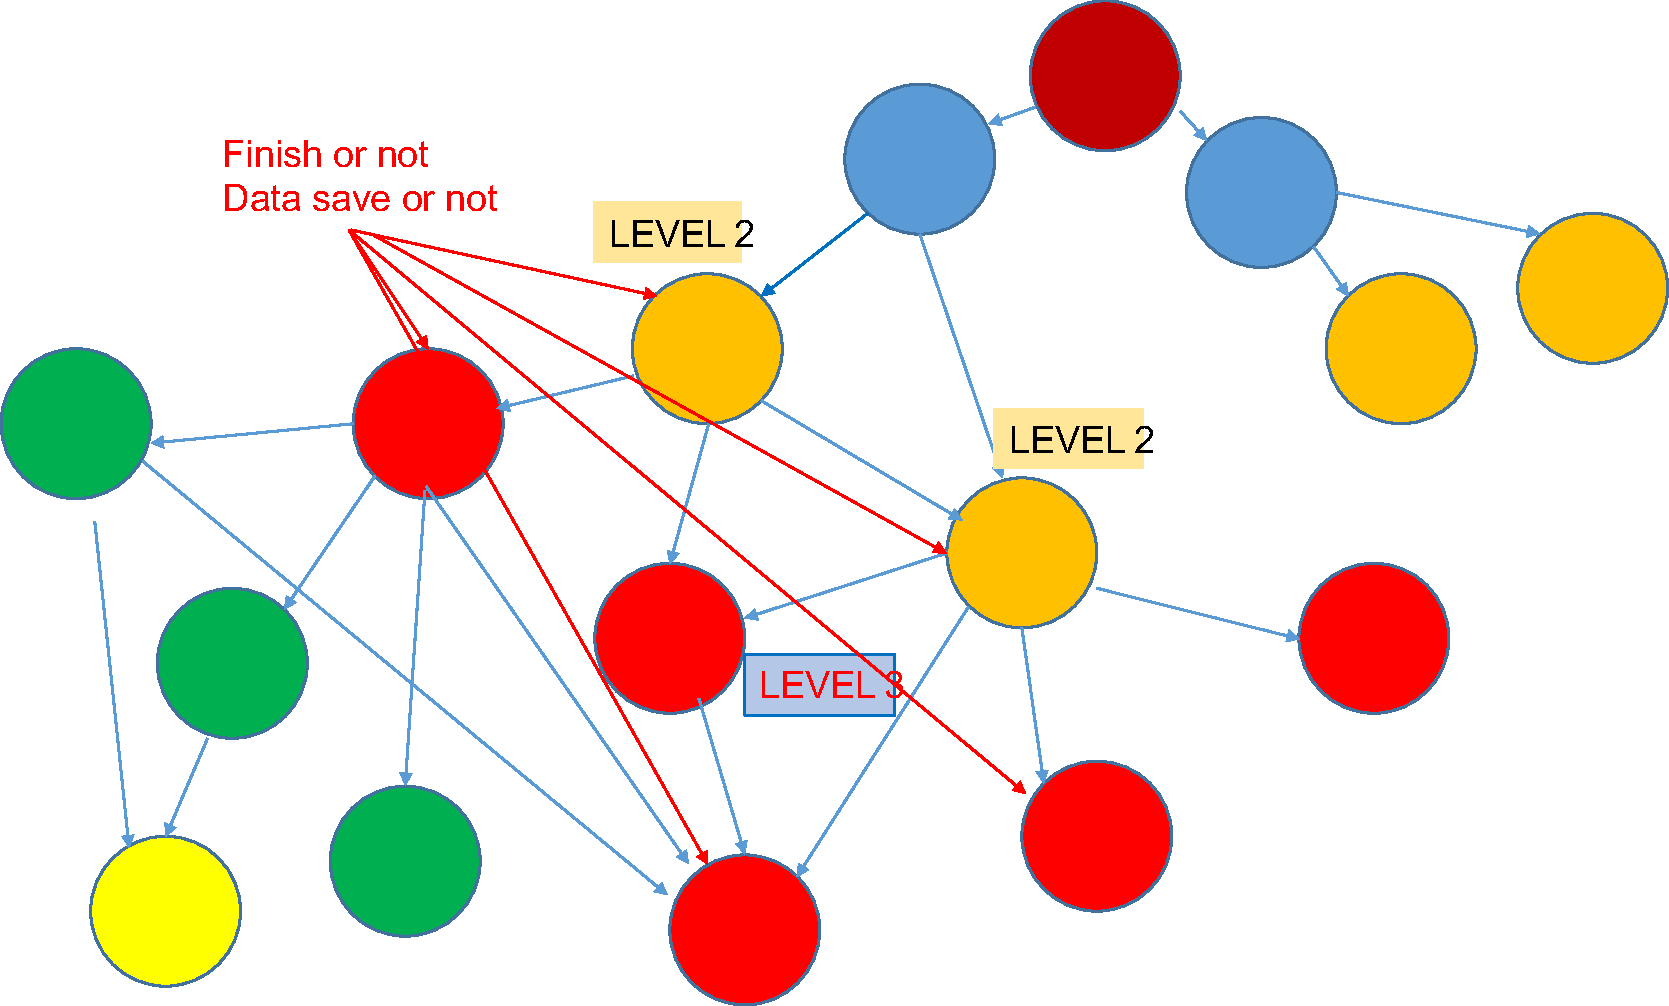
\includegraphics[width=5.in]{fig/exit-branch.pdf}
	\caption{Exiting Parallel Branch.}
	\label{fig:exit}
\end{figure*}

\subsection{Check Pointing}

\subsection{Scheduler for YML/MPI}
\section{Demand for MPI Correction Mechanism}

MUST\footnote{https://tu-dresden.de/zih/forschung/projekte/must} detects usage errors of the Message Passing Interface (MPI) and reports them to the user. As MPI calls are complex and usage errors common, this functionality is extremely helpful for application developers that want to develop correct MPI applications. This includes errors that already manifest - segmentation faults or incorrect results - as well as many errors that are not visible to the application developer or do not manifest on a certain system or MPI implementation.

To detect errors, MUST intercepts the MPI calls that are issued by the target application and evaluates their arguments. The two main usage scenarios for MUST arise during application development and when porting an existing application to a new system. When a developer adds new MPI communication calls, MUST can detect newly introduced errors, especially also some that may not manifest in an application crash. Further, before porting an application to a new system, MUST can detect violations to the MPI standard that might manifest on the target system. MUST reports errors in a log file that can be investigated once the execution of the target executable finishes.
\section{Conclusion}

\clearemptydoublepage
\backmatter

\clearemptydoublepage